\documentclass[conference]{IEEEtran}
\IEEEoverridecommandlockouts
% The preceding line is only needed to identify funding in the first footnote. If that is unneeded, please comment it out.
%Template version as of 6/27/2024

\usepackage{cite}
\usepackage{amsmath,amssymb,amsfonts}
\usepackage{algorithmic}
\usepackage{graphicx}
\usepackage{textcomp}
\usepackage{xcolor}
\def\BibTeX{{\rm B\kern-.05em{\sc i\kern-.025em b}\kern-.08em
    T\kern-.1667em\lower.7ex\hbox{E}\kern-.125emX}}
\begin{document}

\title{Autonomous Farm Sprayer: an efficient spray application approach to common agricultural problems  \\
}

\author{\IEEEauthorblockN{Justin Finn}
\IEEEauthorblockA{\textit{dept. name of organization (of Aff.)} \\
\textit{University of Tennessee at Martin} \\
Martin, TN USA \\
Justinfinn2891@gmail.com}
\and
\IEEEauthorblockN{Thomas Paxton}
\IEEEauthorblockA{\textit{dept. of Engineering} \\
\textit{University of Tennessee at Martin} \\
Martin, TN USA \\
TPaxton@ut.utm.edu}
\and
\IEEEauthorblockN{Jesse Warren}
\IEEEauthorblockA{\textit{dept. name of organization (of Aff.)} \\
\textit{University of Tennessee at Martin}\\
City, Country \\
JWarre46@ut.utm.edu}
\and
\IEEEauthorblockN{Arden Stanley}
\IEEEauthorblockA{\textit{dept. name of organization (of Aff.)} \\
\textit{University of Tennessee at Martin}\\
City, Country \\
astanle8@ut.utm.edu}
}

\maketitle

\begin{abstract}
Efficient and targeted weed management is a critical challenge in modern agriculture, as conventional blanket pesticide applications increase chemical usage, cost, and environmental impact. This project presents an autonomous ground vehicle capable of preventing potential waste and financial issues. With the use of various sensors such as light detection and ranging sensor or LiDAR and a global navigation satellite system module or GNSS, the vehicle will be able to traverse through the rough terrain of the farm plot and simultaneously run a real-time weed identification and classification system using YOLO (You Only Look Once) deep learning framework integrated with a camera-based vision pipeline to achieve high mAH and iOP accuracy. The system is designed to continuously capture images along an autonomously created navigation path and perform real-time object detection to identify weed species within a field of view. Detected weeds are spatially localized and classified with high inference speed, enabling immediate decision-making for precision spraying. Upon successful classification, control commands are generated to activate a pesticide spraying mechanism exclusively at weed locations, minimizing chemical waste and off-target application. The proposed approach demonstrates the feasibility of combining deep learning-based object detection with autonomous or semi-autonomous agricultural platforms to achieve accurate, scalable, and environmentally sustainable weed control. This system highlights the potential of real-time computer vision and robotics to enhance precision agriculture through intelligent perception and actuation. \end{abstract}


\section{Introduction}


\subsection{Project Objective}
For this project, we utilize a supervised learning approach by training a custom dataset obtained from Roboflow with over 1200 images of various of weeds in the local climate within YOLO (You Only Look Once) to accurately identify and classify multiple types of weeds in real time. YOLO is a framework that directly outputs position and category of bounding boxes through its convolutional neural network. The team can later use this information with OpenCV to visually record our results. The purpose of this is to enable precise weed detection, activating a pesticide spraying mechanism when a target weed is identified. This project’s primary objective is to reduce any unnecessary pesticide exposure to crops, mitigating plant damage while maintaining effective weed control in agricultural fields. Excessive pesticide application can decrease the quality of the crop, increase farm expenses in pesticide and negatively impact the surrounding environment; therefore, the application of targeted spraying is crucial for sustainable and efficient agricultural principles and practices. Cost and crop quality are two heavily considered aspects of the design of the system. Pesticides are a common expense for farmers and improper use can comprise plant growth and yield. By limiting the deployment of pesticide primarily to specific weed locations can reduce chemical usage while preserving the quality of the crops. Our approach will help contribute to the improvement of environmentally responsible farming operations. During this project, we will also be comparing the different versions of the YOLO framework; between versions YOLOv5, YOLOv8 and YOLOv11. The team will be comparing the speed and object detection accuracy, to see which version will best work with our dataset. The components essential for navigating through the tested fields require three complementary navigational modules: an intertial measurement unit or IMU, a global navigation satellite system or GNSS, and a 2D light detection and ranging sensor or LiDAR. The 2D LiDAR sensor provides real-time obstacle detection and robotic perception, supporting the safety and reliable navigation through rough and cluttered terrains. The GNSS module  fused with the IMU module, ensures accurate pose updates and supports path planning as the robot systematically scans the field. These three modules and their integration allows the robot to maintain consistent coverage while adapting to any dynamic changes in its surrounding environment.

\subsection{Related Work}

An evolution of changes arose from YOLO as early as its versions from YOLOv1 to YOLOv5 and immense differences from v5 to v8. Major improvements produced the version that will be using today from YOLOv2 adding K-means, YOLOv3’s addition with mutli-scale detection to v5 which involved flexible control of model size \cite{b1}. However, it is important to note the immense speed and capabilities that YOLOv8 has, especially with dealing with immeasurable speed. Although YOLOv11 is a lot more accurate when identifying different classified data\cite{b2}, YOLOv8 is known for its speed in identifying different elements. Because of this, we have decided to use YOLOv8 for our project.

Along with image-based detection, agricultural autonomy and obstacle avoidance is an important topic in current research. Many of the design decisions chosen for this project have been researched and implemented in previous and related designs. Perception sensors such as LiDAR modules and sensor fusion for real time pose updates are the standard for autonomy in the agricultural industry\cite{b3}. Although not directly used during design and testing of the vehicle, many of the control techniques and optimizations have been researched and tested heavily for use in agricultural processes\cite{b4}.


\section{Materials and Methods}

\subsection{Platform Design}
The team concluded that the best approach with respect to the budget and goals set is to utilize a ground vehicle platform capable of traversing the unpredictable terrain of a farm plot. A ground vehicle, as opposed to an aerial vehicle, provides better performance relative to the costs and allows easy additions throughout the testing phases of the project. The platform comprises a 40.5 cm long, 20.25 cm wide, and 8.25 cm tall fabricated aluminum chassis. The choice of aluminum provides the structural rigidity required but keeps the chassis lightweight. A computer-aided design model is provided in Figure 2. The dimensions chosen for the chassis will accommodate all the current components selected and leave extra space for any additional components needed as we refine the project while allowing easy maneuverability between the corn rows. To increase stability, weights were added to the front of the chassis. With the platform fully assembled, the center of gravity is located front to rear, directly in the center of the contact path of the track.

% CAD image of chassis
\begin{figure}[htbp]
\centerline{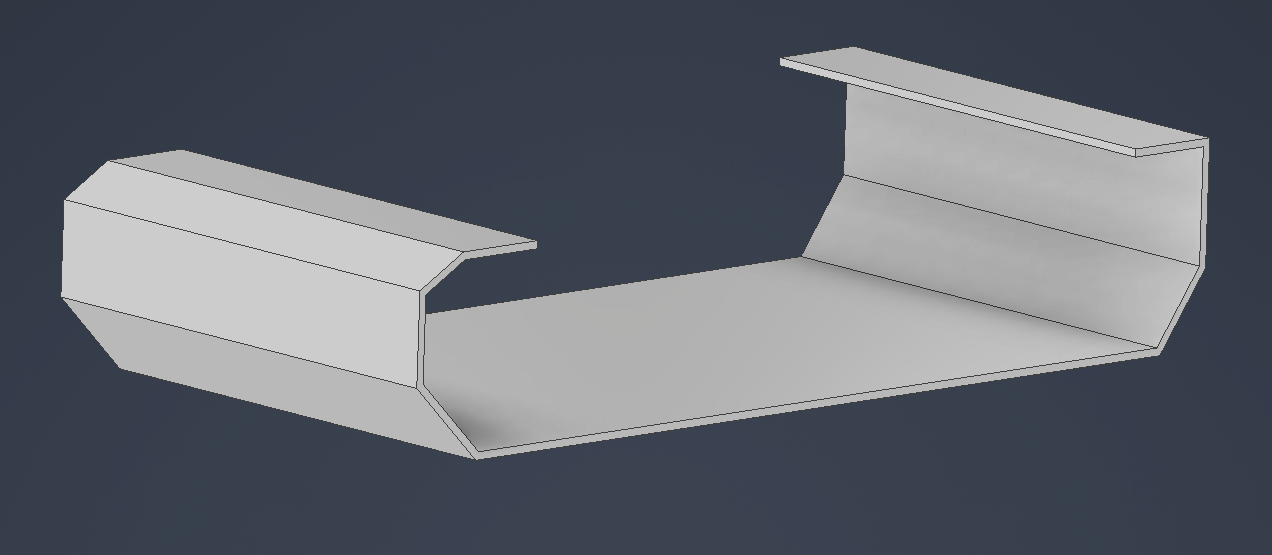
\includegraphics[width=.9\columnwidth]{ChassisCAD.png}}
\caption{CAD model of chassis design.}
\label{fig:CAD_Model}
\end{figure}

\subsection{Electrical System}

The electrical system is broken down into two circuits. The first circuit is powered by a 6000 mAh 3S lithium polymer battery, and provides power for the drive system and, using a buck converter, steps down the battery voltage to 5 volts for the sensor suite and microcontrollers. As a manual override and for ease of use, the vehicle includes the ability to manually be controlled using an ESP32 microcontroller and its Bluetooth capabilities. This allows the use of a Bluetooth controller to manually drive and activate the spraying system remotely. A Teensy 4.1 microcontroller is used as the main controller for most of the systems on the vehicle. The Teensy handles the inputs provided by the sensor suite and Raspberry Pi and sends commands to the drive system and sprayer system. The drive system utilizes 2 single channel Pololu VNH5019 motor drivers to drive the motors. The second circuit encompasses the herbicide sprayer system. This will be powered by a separate 6000 mAh 3S lithium polymer battery and provides power for the solenoids and pump via a 4-channel relay and 1 channel relay respectively.

The sensor suite consists of 2 main areas. The first area is the autonomous driving sensor suite, and the second area is the weed detection system. The autonomous driving suite consists of RP LiDAR C1 for perception of the corn rows and collision avoidance. Handling the pose of the robot is a fused GNSS module and 10 degree of freedom IMU with a compass. The wiring schematic referenced here is shown in Figure 2. As for the AI sensor suite, the project includes a Raspberry Pi single board computer and a Raspberry Pi AI camera.

% Schematic image
\begin{figure}[htbp]
\centerline{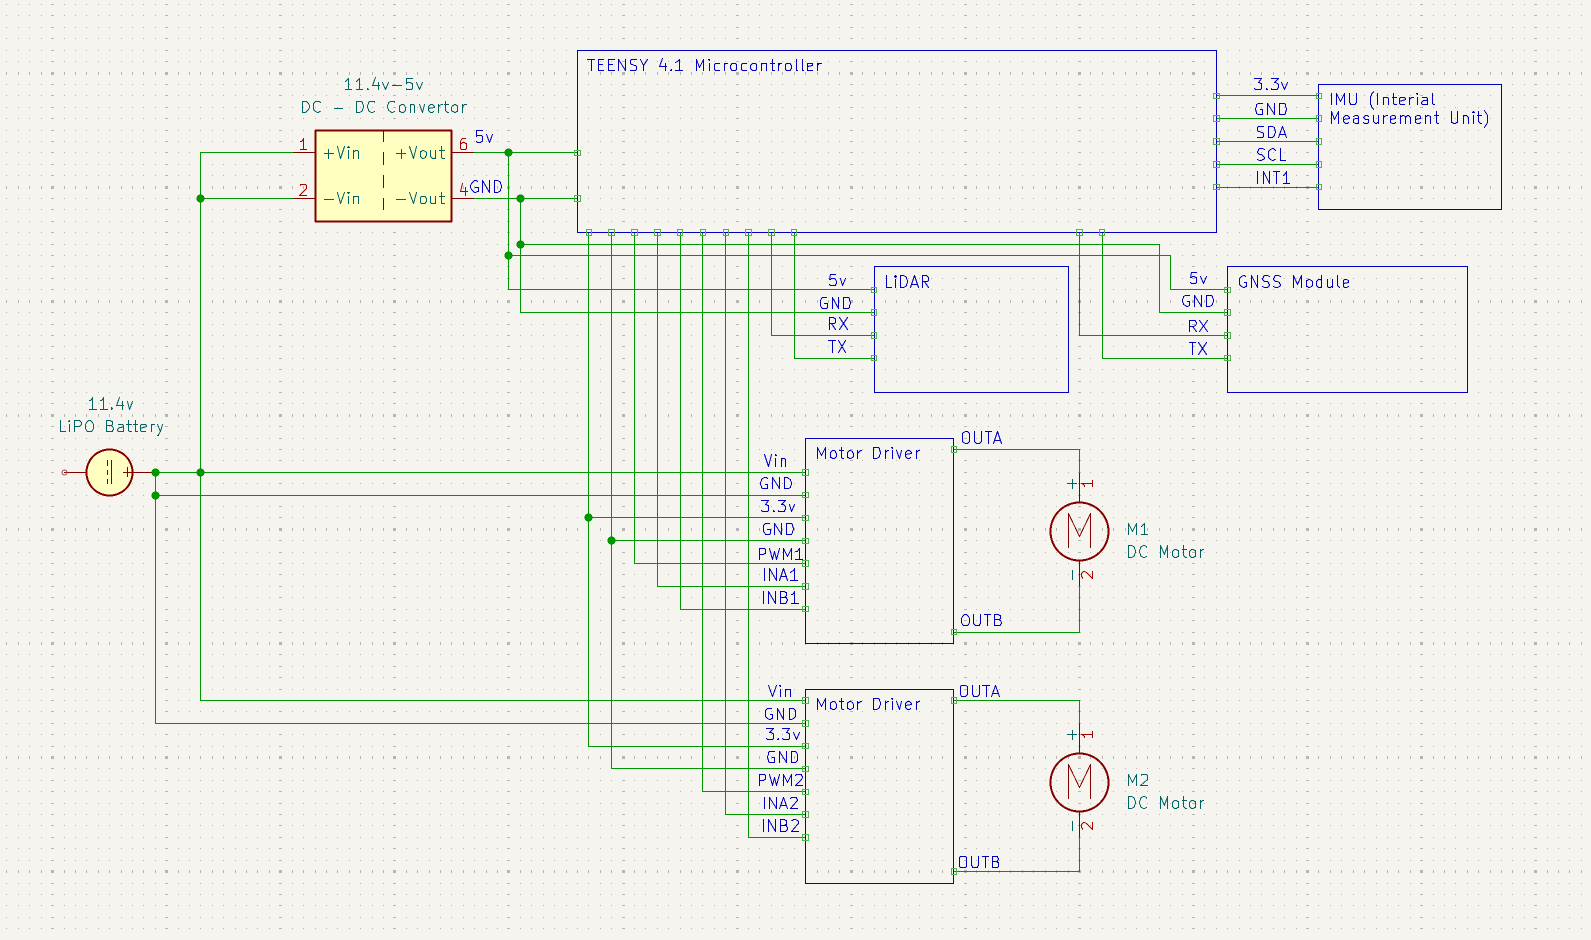
\includegraphics[width=.9\columnwidth]{Schematic.png}}
\caption{Wiring diagram of sensor suite.}
\label{fig:Wiring_Diagram}
\end{figure}

\subsection{AI Weed Detection and YOLO Architecture}

To detect weeds and apply pesticide only where needed, our original plan was to use a convolutional neural network (CNN) built in PyTorch to identify weeds in images taken from the field. The CNN would be trained on a labeled dataset of weed images so it could learn basic visual features such as leaf shape, texture, and color. After training, the model would classify images in real time and trigger pesticide spraying when weeds were detected, helping reduce overspray. However, as the project developed, we realized that this approach would not provide the speed and precision required for a moving robotic system. A basic CNN is mainly designed to classify entire images and does not easily provide the exact location of weeds within the camera view, which is necessary for accurate spraying while the robot is in motion. To improve performance and reliability, we transitioned to using the YOLO (You Only Look Once) object detection framework, specifically YOLOv8. YOLOv8 is designed for real-time detection and can both identify weeds and determine their position in a single step. This allows the system to quickly and accurately detect weeds as the robot moves through the field and apply pesticide only where needed. By switching to YOLOv8, the system achieves faster detection, better accuracy, and more precise spraying, making it better suited for real-world field conditions and efficient pesticide applications. The team aims to use YOLO to turn the object detection problem into a regression problem. The architecture of YOLO consists of 24 convolutional layers as well as 4 pooling layers and 2 fully connected layers. YOLO will resize the input image from its respective size to 448 pixels by 448 pixels. The different versions of YOLO that we test will display different constant input size changes. The activation function for YOLO is ReLU until the last layer which uses a linear activation function [3]. The key measurements we hope to retain from this original architect that have remained intact throughout the various versions of YOLO are the quantitative measurements. It is crucial, especially when dealing with small objects such as weeds, to record the average precision, to calculate the area under the precision vs recall curve, and intersection over union (IOU), to calculate localization accuracy, for each process of the model [4]. These measurements will be held as a value resembling success in our model. It will also be important to record the confidence score and class probability for each bounding box.

The traditional approach to YOLO came from Joseph Redmon and his colleagues Santosh Divvala, Ross Girshick, and Ali Farhad. The purpose of YOLO was to exceed the expectations of average real-time image detectors at the time. YOLO takes the original object detection problem and treats it as a regression problem, dealing with bounding boxes and associated possibilities to each detected image using a trained CNN [3]. The success of YOLO comes from its simple architecture which gives speed, detection accuracy, and good generalization when it comes to identifying images. Because of this, the traditional YOLO framework can achieve 45 frames per second while doubling the average precision mAP comparable to other real time systems.

% CNN photo 1
\begin{figure}[htbp]
\centerline{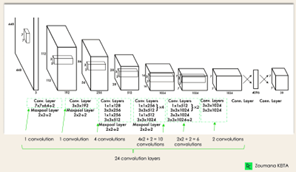
\includegraphics[width=.9\columnwidth]{CNN1.png}}
\caption{Architecture of the traditional YOLO framework.}
\label{fig:CNN1}
\end{figure}

It is important to observe the key differences between the architecture and performance of the various versions of YOLO to incorporate the fastest one for our results. The two versions we tested includes YOLOv8 and YOLOv11. With the precise measurements we need to achieve to train our model to identify various types of weeds based on color, shape and orientation, models such as YOLOv7 and below won’t be able to manage this data. There are various limitations with these previous versions such as struggling to detect small objects, especially from different scales, and the models are overall computationally intensive [4]. To test the two separate models, YOLOv8 and YOLOv11, we are using a dataset containing 4200 pictures of weeds to obtain measurable results and begin the training process on our autonomous farm sprayer.

\subsection{Sprayer Mechanism}

The spraying mechanism is based on the industry standard boom arm setup seen on conventional sprayer systems that has been scaled down to fit the test chassis. The boom arm is constructed of PVC piping mounted with 3D printed mounts and tee connections. Given the weight of all components mounted to the boom arm, the PVC piping is more than capable of supporting the loads. The boom arm measures 30 cm tall with 20.25 cm of rear offset which should clear the height of the young corn plants while providing clearance from spraying the chassis itself. As the platform is processing one row at a time, the width of the boom arm matches the width of the corn rows at 76.2 cm across but is easily adjustable to allow compatibility with different row widths.

The selection of sprayer components was driven by budget concerns and ease of testing. For controlling the precision spraying system, the vehicle uses 4 Adafruit 12-volt solenoids, mounted using adjustable 3D printed mounts on the boom arm, allowing individual actuation of spray zones. Mounted directly to the end of the solenoids are 3D printed adapters that fit a 68.94 kPa check valve to prevent low pressure dribbling after the solenoid closes. Along with the check valve, the adapter was designed to accept standard off-the-shelf TeeJet quick change nozzles. This allows quick and easy adjustments when testing different spray patterns to best suit the application. A Delavan 3.785 LPM pump is connected to the solenoids using 3/8" high pressure PVC hose and tee fittings providing 275 kPa of pressure. During initial testing, adequate flow was provided with all 4 solenoids activated at the same time using the current nozzle selection. Fluid storage is handled with a 1.89 liter HPDE tank mounted in line with the center of gravity to ensure no drastic changes to the stability as the fluid level drops.

For controlling the components of the sprayer mechanism, the system utilizes 5 general purpose input output (GPIO) pins on the Teensy 4.1 microcontroller. 4 pins are connected to a 4-channel relay used solely for controlling the activation of the solenoids. The final pin is connected to a single channel relay providing fine control of the pump activation. Pressure is controlled internally by the Delavan pump.

\subsection{Autonomous Path Planning}

To achieve full autonomy for the vehicle, the system employs the use of a GNSS module fused with an IMU module and a two-dimensional LiDAR scanner to allow the autonomous vehicle to detect its current pose and the environment surrounding itself. Given the environment the vehicle will be built to traverse, the team specifically designed the software to be capable of traversing through a field between rows of corn. This is achieved by the use of pure pursuit pathing towards waypoints compared to the current pose estimation, which gives the vehicle a set objective to push towards. The LiDAR scanner, mounted to the top of the vehicle, scans in a 360 degree plane and returns both distance values and the angles which they were read from. The scanner will detect the fledgling corn stalks on both sides of the autonomous ground vehicle and recognize them as a wall to avoid. Once a certain distance threshold is exceeded, the vehicle will adjust its position and set a new waypoint, eventually reaching the end of the field. To switch to a different row, the closest stalk is read by the LiDAR and compared to the GNSS module and used as a detect object to pivot itself around until it reaches the start of another row.

In regard to the software, the C++ language was utilized due to familiarity from the project members as well as its low level capabilities and speed. Given the amount of data and need for quick response, we’ve used a microcontroller capable of a 600MHz clock rate, namely the Teensy 4.1, for both the autonomy and sprayer portion of the project.

% Lidar diagram image
\begin{figure}[htbp]
\centerline{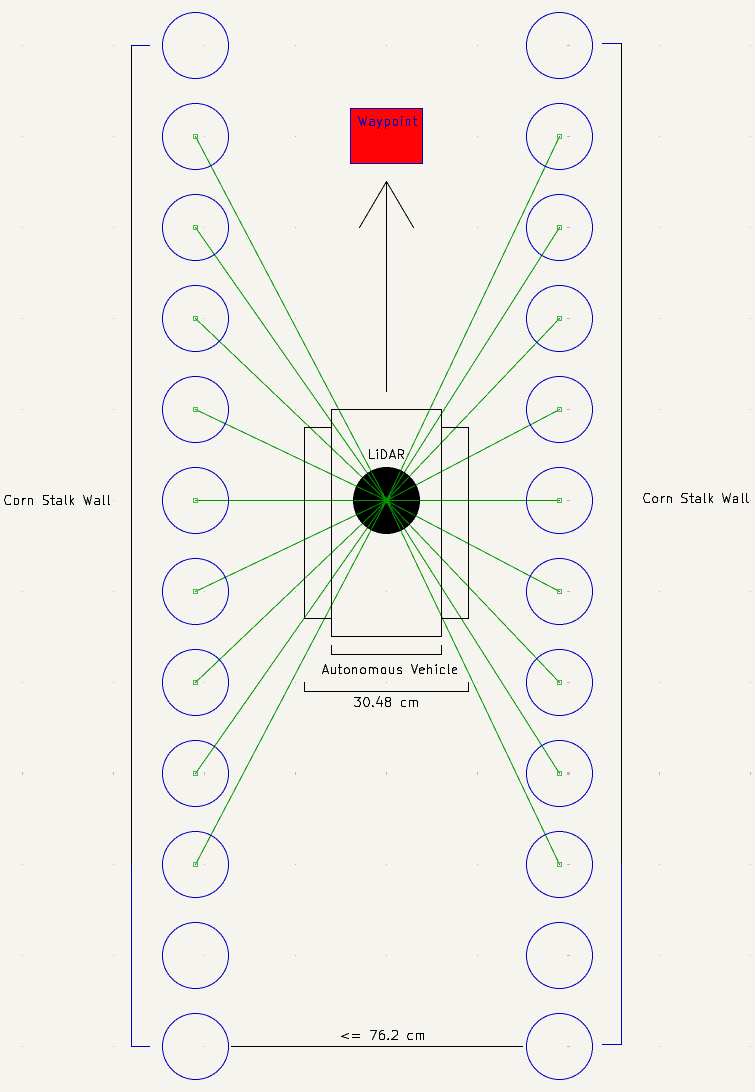
\includegraphics[width=.9\columnwidth]{LidarDiagram.png}}
\caption{Top view of LiDAR scanning process.}
\label{fig:Lidar_Diagram}
\end{figure}

In the attempt to achieve autonomous pathfinding, the project is based on a finite state machine to control different behaviors throughout the traversal of the farm plot. During all states, two systems are always running. Firstly, pose updates are created using a GNSS module and IMU module. These sensors are fused using an extended Kalman filter to enhance accuracy as the vehicle traverses the field. The other system running constantly is the LiDAR scanner. The LiDAR scanner sends a full rotation of data points at a time, and the Teensy 4.1 microcontroller parses the data and stores it in order for the different states to manipulate the data for the task at hand.  The state machine consists of 2 main states with several substates running within the main states. The first of the two main states includes \textit{Manual Drive}. During \textit{Manual Drive}, all commands sent to the various systems are controlled via a Bluetooth controller. From this controller, the user can command all 4 solenoids and the individual banks of the differential drive system. This allows full manual intervention if any issues are detected during testing. Along with this, rather than setting the vehicle in the field, we can drive it to its starting position before activating full autonomy.

The second main state is the \textit{Auto Drive} state. This state controls all of the inputs and outputs of the vehicle with full autonomy. Within this state there are several substates. The substates include \textit{InbetweenRows}, \textit{End of Row}, \textit{Turning}, \textit{Aligning}, and \textit{Safety Stop}.

The first state and most common state, \textit{Inbetween Rows}, handles most of the calculations and outputs to drive the vehicle down the center path of the current row. This is done taking the LiDAR data and filtering it into 2 sets, one for the left side row and one for the right-side row. After the data is separated, a random sample consensus or RANSAC algorithm is applied to both sets providing two estimations for the corn rows on either side. After the valid rows are established, a waypoint is created and stored for the vehicle to drive to. After reaching the end of the row, lidar hits are checked to the left and right and if none are found, the vehicle is moved to the \textit{End of Row} state. During the \textit{End of Row} state, the vehicle stores its current heading and then drives a set distance outside of the row and attempts to find the next row before transitioning to the next state. The next state is \textit{Turning}. During this state, the vehicle finds the next row and makes a constant radius turn towards the next row. Once the compass reads 180 degrees from the previously stored heading and detects the opening to the new row, the vehicle transitions to the \textit{Aligning} state. During the \textit{Aligning} state, the vehicle prepares to center into the new row before looking for hits on the left and right side of the vehicle causing it to transfer to the \textit{Inbetween Rows} state and then repeating the cycle until completion. During any state, the vehicle is constantly checking the lidar data and pose estimatioms to ensure the vehicle is not outside of safe operating ranges. If the vehicle detects a collision or detects pose outside of the set threshold, it switches to the \textit{Safety Stop} state. During this state it recalls the most recent waypoint and attempts to reverse back to the waypoint. Once the waypoint is reached, the vehicle switches back to \textit{Inbetween Rows} state and retries. If no motion is detected after a set amount of time, the vehicle switches back to \textit{Manual Drive} state. A state diagram is provided below for the Auto Drive substates.

% State Machine image
\begin{figure}[htbp]
\centerline{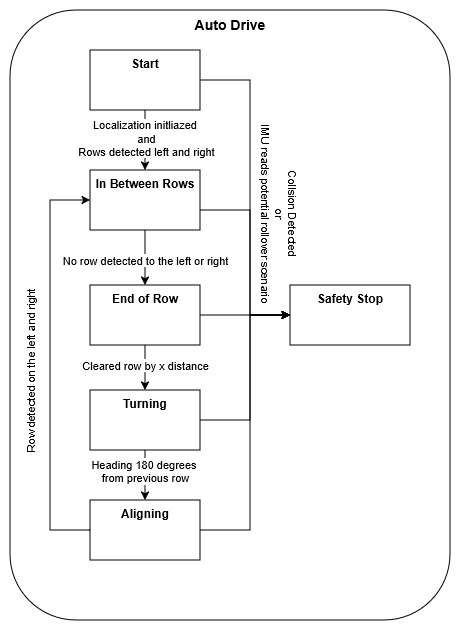
\includegraphics[width=.9\columnwidth]{AutoDriveOnly.png}}
\caption{State Diagram for Auto Drive substate.}
\label{fig:StateMachine}
\end{figure}

\section{Results}

The dataset for training our YOLO model was curated and augmented using Roboflow and exported in YOLO format. Training was conducted on Google Colab using the Ultralytics YOLOv8 framework with an input resolution of 640×640 over 50 epochs. The dataset used in this study consists of 1,200 annotated images, which were divided into 840 training images, 240 validation images, and 120 test images, corresponding to a 70/20/10 split. All images were annotated using axis-aligned bounding boxes in YOLO format for object detection.

% CNN image 2
\begin{figure}[!htbp]
\centerline{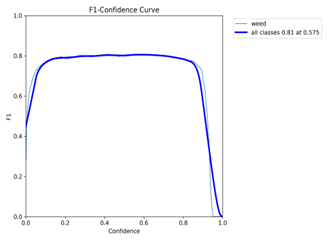
\includegraphics[width=.9\columnwidth]{CNN2.png}}
\caption{F1 Confidence Curve for trained model from Google Colab results.}
\label{fig:CNN2}
\end{figure}

The F1–confidence curve shows how changing the confidence threshold affects the model’s performance. The model reaches its best F1 score, about 0.81, at a confidence value of 0.575, which represents a good balance between precision and recall. The performance stays fairly consistent across a wide range of confidence levels, showing that the model is stable and reliable. At lower confidence values, the model detects more objects but also produces more false positives, while at higher confidence values it misses more weeds, causing performance to drop. Based on this trend, a confidence threshold between 0.55 and 0.60 works best for practical weed detection.

% CNN image 3
\begin{figure}[!htbp]
\centerline{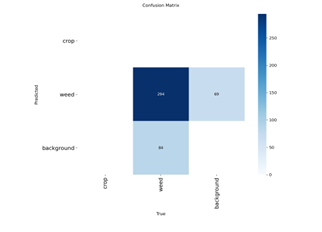
\includegraphics[width=.8\columnwidth]{CNN3.png}}
\caption{Confusion Matrix for trained model from Google Colab results.}
\label{fig:CNN3}
\end{figure}
\smallskip
% CNN image 4
\begin{figure}[!htbp]
\centerline{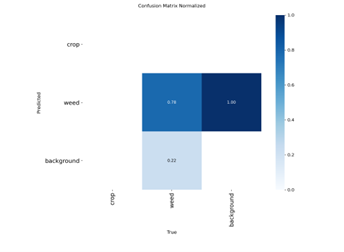
\includegraphics[width=.8\columnwidth]{CNN4.png}}
\caption{Normalized Confusion Matrix for trained model from same results .}
\label{fig:CNN4}
\end{figure}

The confusion matrix evaluated on the test dataset shows strong classification performance for our weed detection model, with the majority of weed instances correctly identified. Specifically, 294 weed instances were correctly classified, indicating great feature learning for the target class. A portion of weed samples (84 instances) were misclassified as background, suggesting that smaller or visually ambiguous weeds were occasionally missed. Additionally, 69 background instances were incorrectly classified as weeds, representing false positives that may result from background vegetation or soil textures resembling weed characteristics. Notably, minimal confusion was observed between crop and weed classes, indicating effective class separation. Overall, the confusion matrix confirms the model’s reliability for weed detection while highlighting opportunities to reduce background-related misclassifications through additional training data or refined annotations.

% CNN image 5
\begin{figure}[!htbp]
\centerline{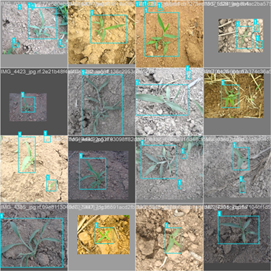
\includegraphics[width=.9\columnwidth]{CNN5.png}}
\caption{Validity for example detection of various weed plants.}
\label{fig:CNN5}
\end{figure}

Figure 9 shows example detections from the training and validation datasets. The model is able to correctly identify weed plants across different soil types, lighting conditions, and plant sizes. Most weeds are tightly enclosed by bounding boxes, indicating accurate localization. Some smaller or partially visible weeds are harder to detect, but overall, the model consistently identifies the target plants. These examples show that the model learned meaningful visual features and generalized well to unseen validation images.

% CNN image 6
\begin{figure}[!htbp]
\centerline{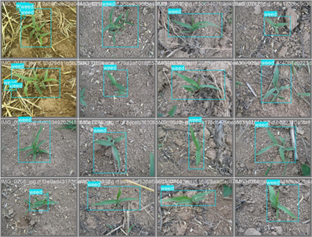
\includegraphics[width=.9\columnwidth]{CNN6.png}}
\caption{Final detection of various weed plants.}
\label{fig:CNN6}
\end{figure}


\section{Discussions}


\subsection{Challenges and System Limitations}

One of the main limitations of our prototype is size. Current spraying methods primarily use large and expensive spraying equipment with the ability to encompass many rows at a time. As the project focuses more on testing rather than a production-ready vehicle, the vehicle was designed much smaller than the industry standard. This allows us to allocate more of our budget towards autonomy and other various systems included in the project. Along with this, using primarily consumer grade components created roadblocks as the project progresses through its testing phases. This issue was most prevalant with our LiDAR module. As the laser was limited on power, operations during brighter days led to noisy data as the lidar module had troubles gathering data.

\subsection{Future Work}

In the future, there are many improvements that could be made to better the performance of the vehicle. One of the easiest improvements planned includes adding on-the-fly height adjustment of the boom arm. The closer the nozzle can get to the source of the weeds the less likely overspray will occur further decreasing environmental impact of spraying chemicals. Along with this, as there has been many improvements with RANSAC line fitting algorithms, the vehicle could benefit from testing with different lightweight forms of RANSAC\cite{b7}.

\section{Conclusions}

This project showcases the growing role that robotic systems can become involved with improving the efficiency, sustainability, and precision of modern agricultural life. By cultivating and designing an autonomous vehicle capable of detecting and spraying weeds, we demonstrated a cost-effective practical alternative to the traditional blanket pesticide approach that often involves the unnecessary use of excess chemicals, increased costs and negative effects on the environment. Our approach’s ability to identify weeds in real time with the use of YOLO and apply herbicide only where it needed shows how precision agricultural technologies can address these common issues while preserving the overall health of the corn plots and quality of the soil.


A key contribution to this project is the successful use of real-time computer vision with a mobile robot operating in a realistic and rough environment. The use of YOLO, specifically YOLOv8, and its framework enables fast and reliable weed classification, augmentation and identification, even as the robot roams around its vast and ever-changing environment. By comparing multiple YOLO versions, we were able to choose the best version needed for detection speed and accuracy to produce the finest results for our robot. The results given show that modern deep learning models can generalize well to unseen field data, making them suitable for on-the-fly decision making in several common agricultural tasks. This reinforces the idea that these modern vision-based approaches are no longer just limited and controlled in laboratory settings but can function effectively in dynamic and practical environments regardless of several variables.


Beyond the vision of our robot, the project also focusses heavily on coordinating sensing and navigation. Both the GNSS-based waypoint navigation and LiDAR obstacle detection allow the ground vehicle to repeatedly traverse crop rows while adapting to any change in the environment. This layered approach to autonomy improves reliability and safety while maintaining coverage across the field. The selective spraying mechanism continues to connect perception and action by translating weed detections into precise control of solenoids and pumps, ensuring that chemical application is localized and intentional. Together, these components demonstrate how autonomous systems can close the loop between sensing, decision-making, and physical interaction with the environment.


Overall, this project and its results show how the integration of robotics and artificial intelligence can lead to a more sustainable and economical future for farmers and their practices. By reducing any unnecessary waste of pesticide, maintaining decent quality and health of the crops, this system provides a purposeful approach to the goals of future agricultural solutions. This proposed approach effectively demonstrates the feasibility of combining deep learning-based object detection with autonomous or semi-autonomous agricultural platforms to achieve accurate, scalable, and environmentally sustainable weed control.

\section{References}
\begin{thebibliography}{00}
\bibitem{b1} P. Jiang, D. Ergu, F. Liu, Y. Cai, and B. Ma, ‘A Review of Yolo Algorithm Developments’, Procedia Computer Science, vol. 199, pp. 1066–1073, 2022.
\bibitem{b2} Aboul Ella Hassanien, S. Anand, A. Jaiswal, and P. Kumar, Innovative Computing and Communications, vol. 7. Springer Nature, 2025, pp. 363–372.
\bibitem{b3}H. Wu, X. Wang, X. Chen, Y. Zhang, and Y. Zhang, ‘Review on Key Technologies for Autonomous Navigation in Field Agricultural Machinery’, Agriculture, vol. 15, no. 12, 2025.
\bibitem{b4} Z. Chen et al., ‘A comprehensive review of obstacle avoidance for autonomous agricultural machinery in multi-operational environment’, Artificial Intelligence in Agriculture, vol. 16, no. 1, pp. 139–163, 2026.
\bibitem{b5} Z. Kelta, “YOLO Object Detection Explained: A Beginner’s Guide,” www.datacamp.com, Sep. 2022. https://www.datacamp.com/blog/yolo-object-detection-explained
\bibitem{b6} R. Kundu, “YOLO: Real-Time Object Detection Explained,” www.v7labs.com, Jan. 17, 2023. https://www.v7labs.com/blog/yolo-object-detection.
\bibitem{b7} J. M. Martínez-Otzeta, I. Rodríguez-Moreno, I. Mendialdua, and B. Sierra, ‘RANSAC for Robotic Applications: A Survey’, Sensors, vol. 23, no. 1, 2023.
\end{thebibliography}

\end{document}
